\chapter[Implementering af hardware]{Hardware}

% Vi skriver her om hvordan vi faktisk realiserer det vi har sankket
% om i Hardwaredesignet

\section{Stepmotor driver}
Vi skal som nævnt i afsnittet \titleref{ch:d-hardware} konstruere en
stepmotor driver, med et par integrerede stepmotor drivere. Mere
specefikt anvender vi et par L6208N'ere, hvilket er en DMOS driver til
bipolare stepmotorer. Vi bruger denne driver, da den er simpel at
styre, samt der er mulighed for at lave strømbegrænsning.



\section{Sensorerne}
\fixme{delkredskøb til gaffelsensorerne}

\mnote{
  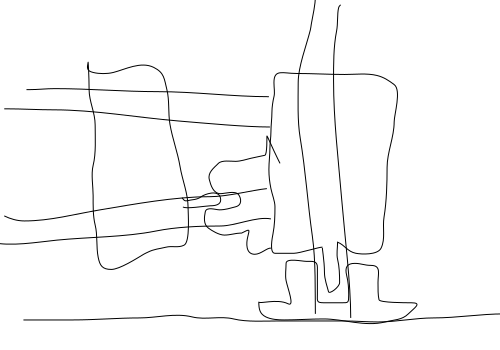
\includegraphics[width=\marginparwidth]{./img/fotogafel-skitse}
  \captionof{figure}{Placering af fotogafler}
  \label{fig:transducer-skitse}
}
\fixme{nick: Illustrationen af sensorerne skal laves rigtigt}

\mnote{
  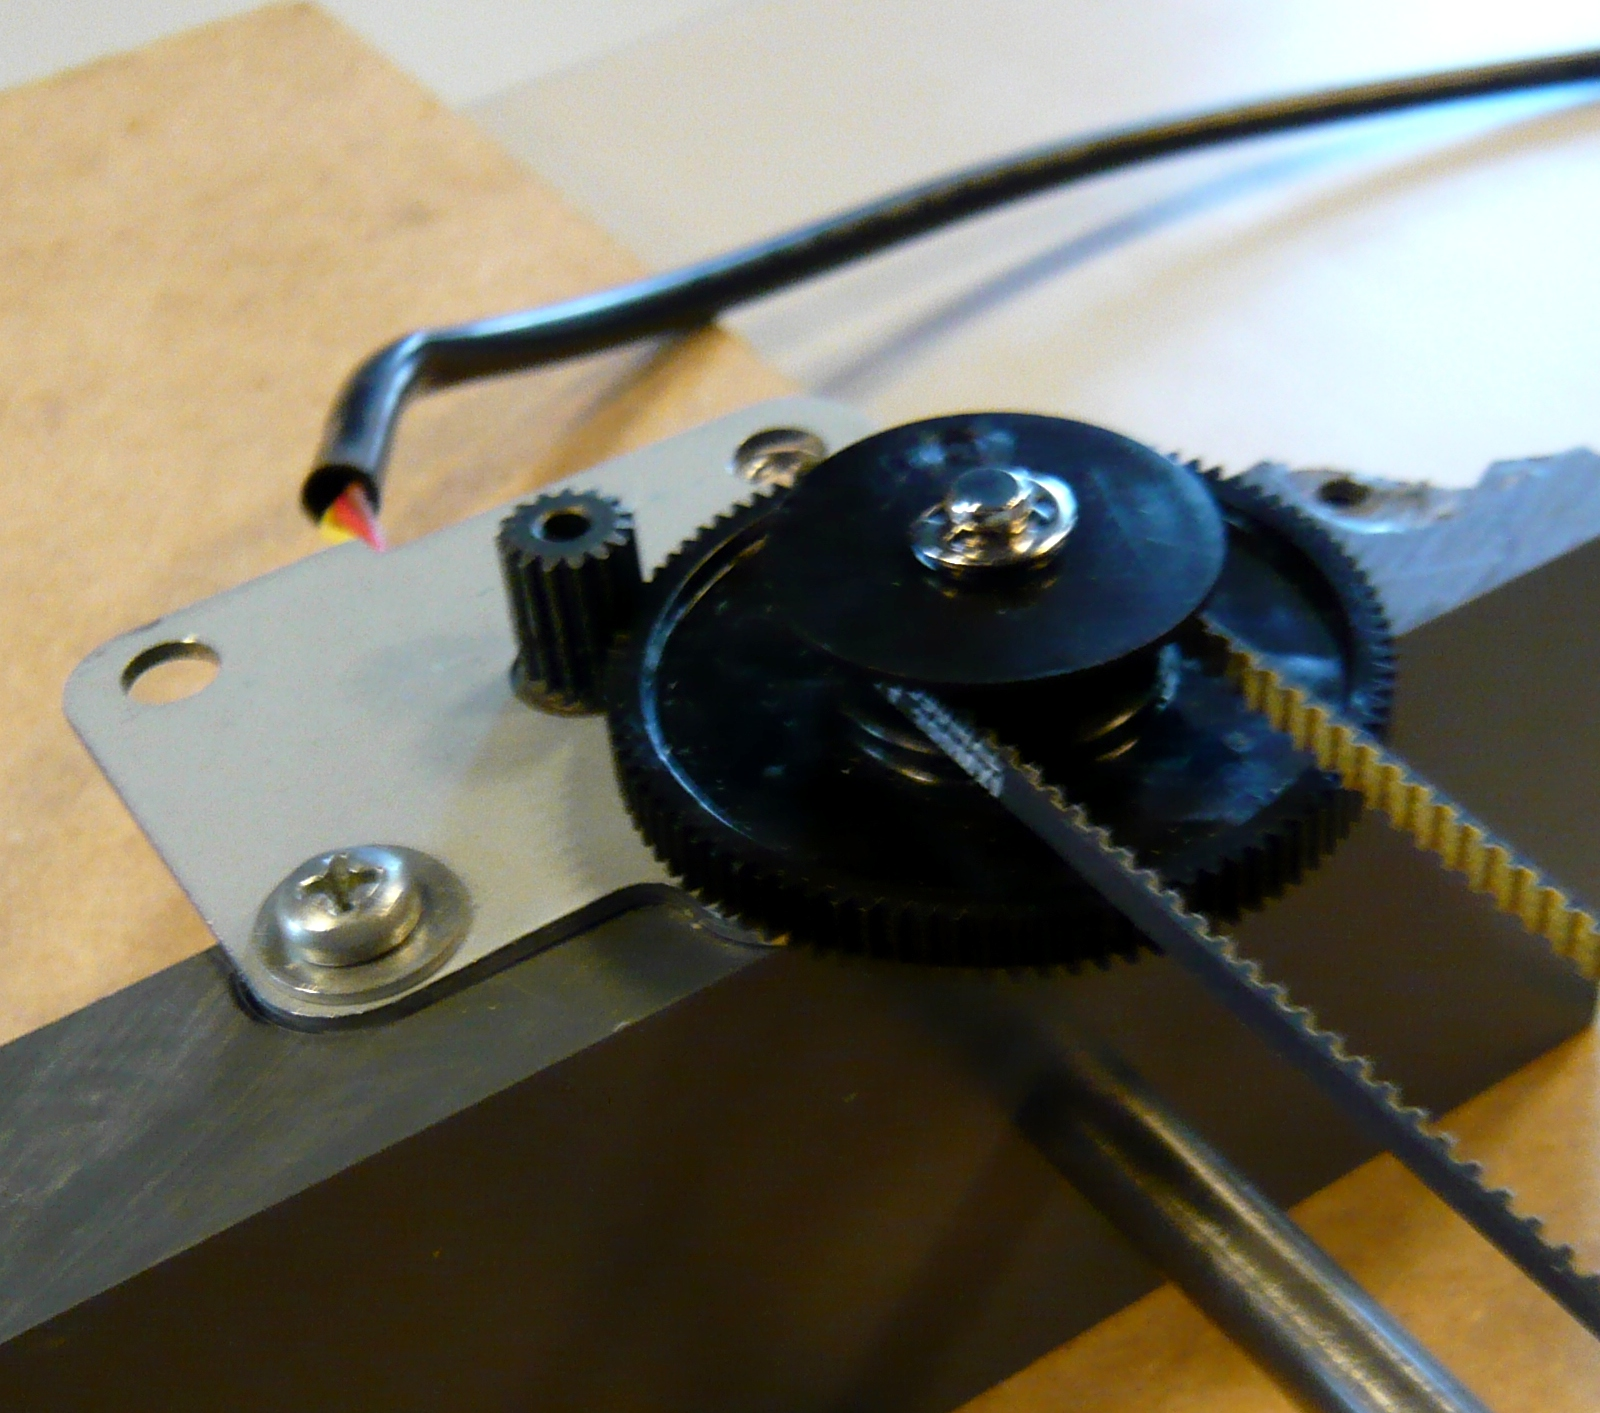
\includegraphics[width=\marginparwidth]{./img/x-motor}
  \captionof{figure}{Billede af x-motoren}
  \label{fig:x-motorimg}
}

\mnote{
  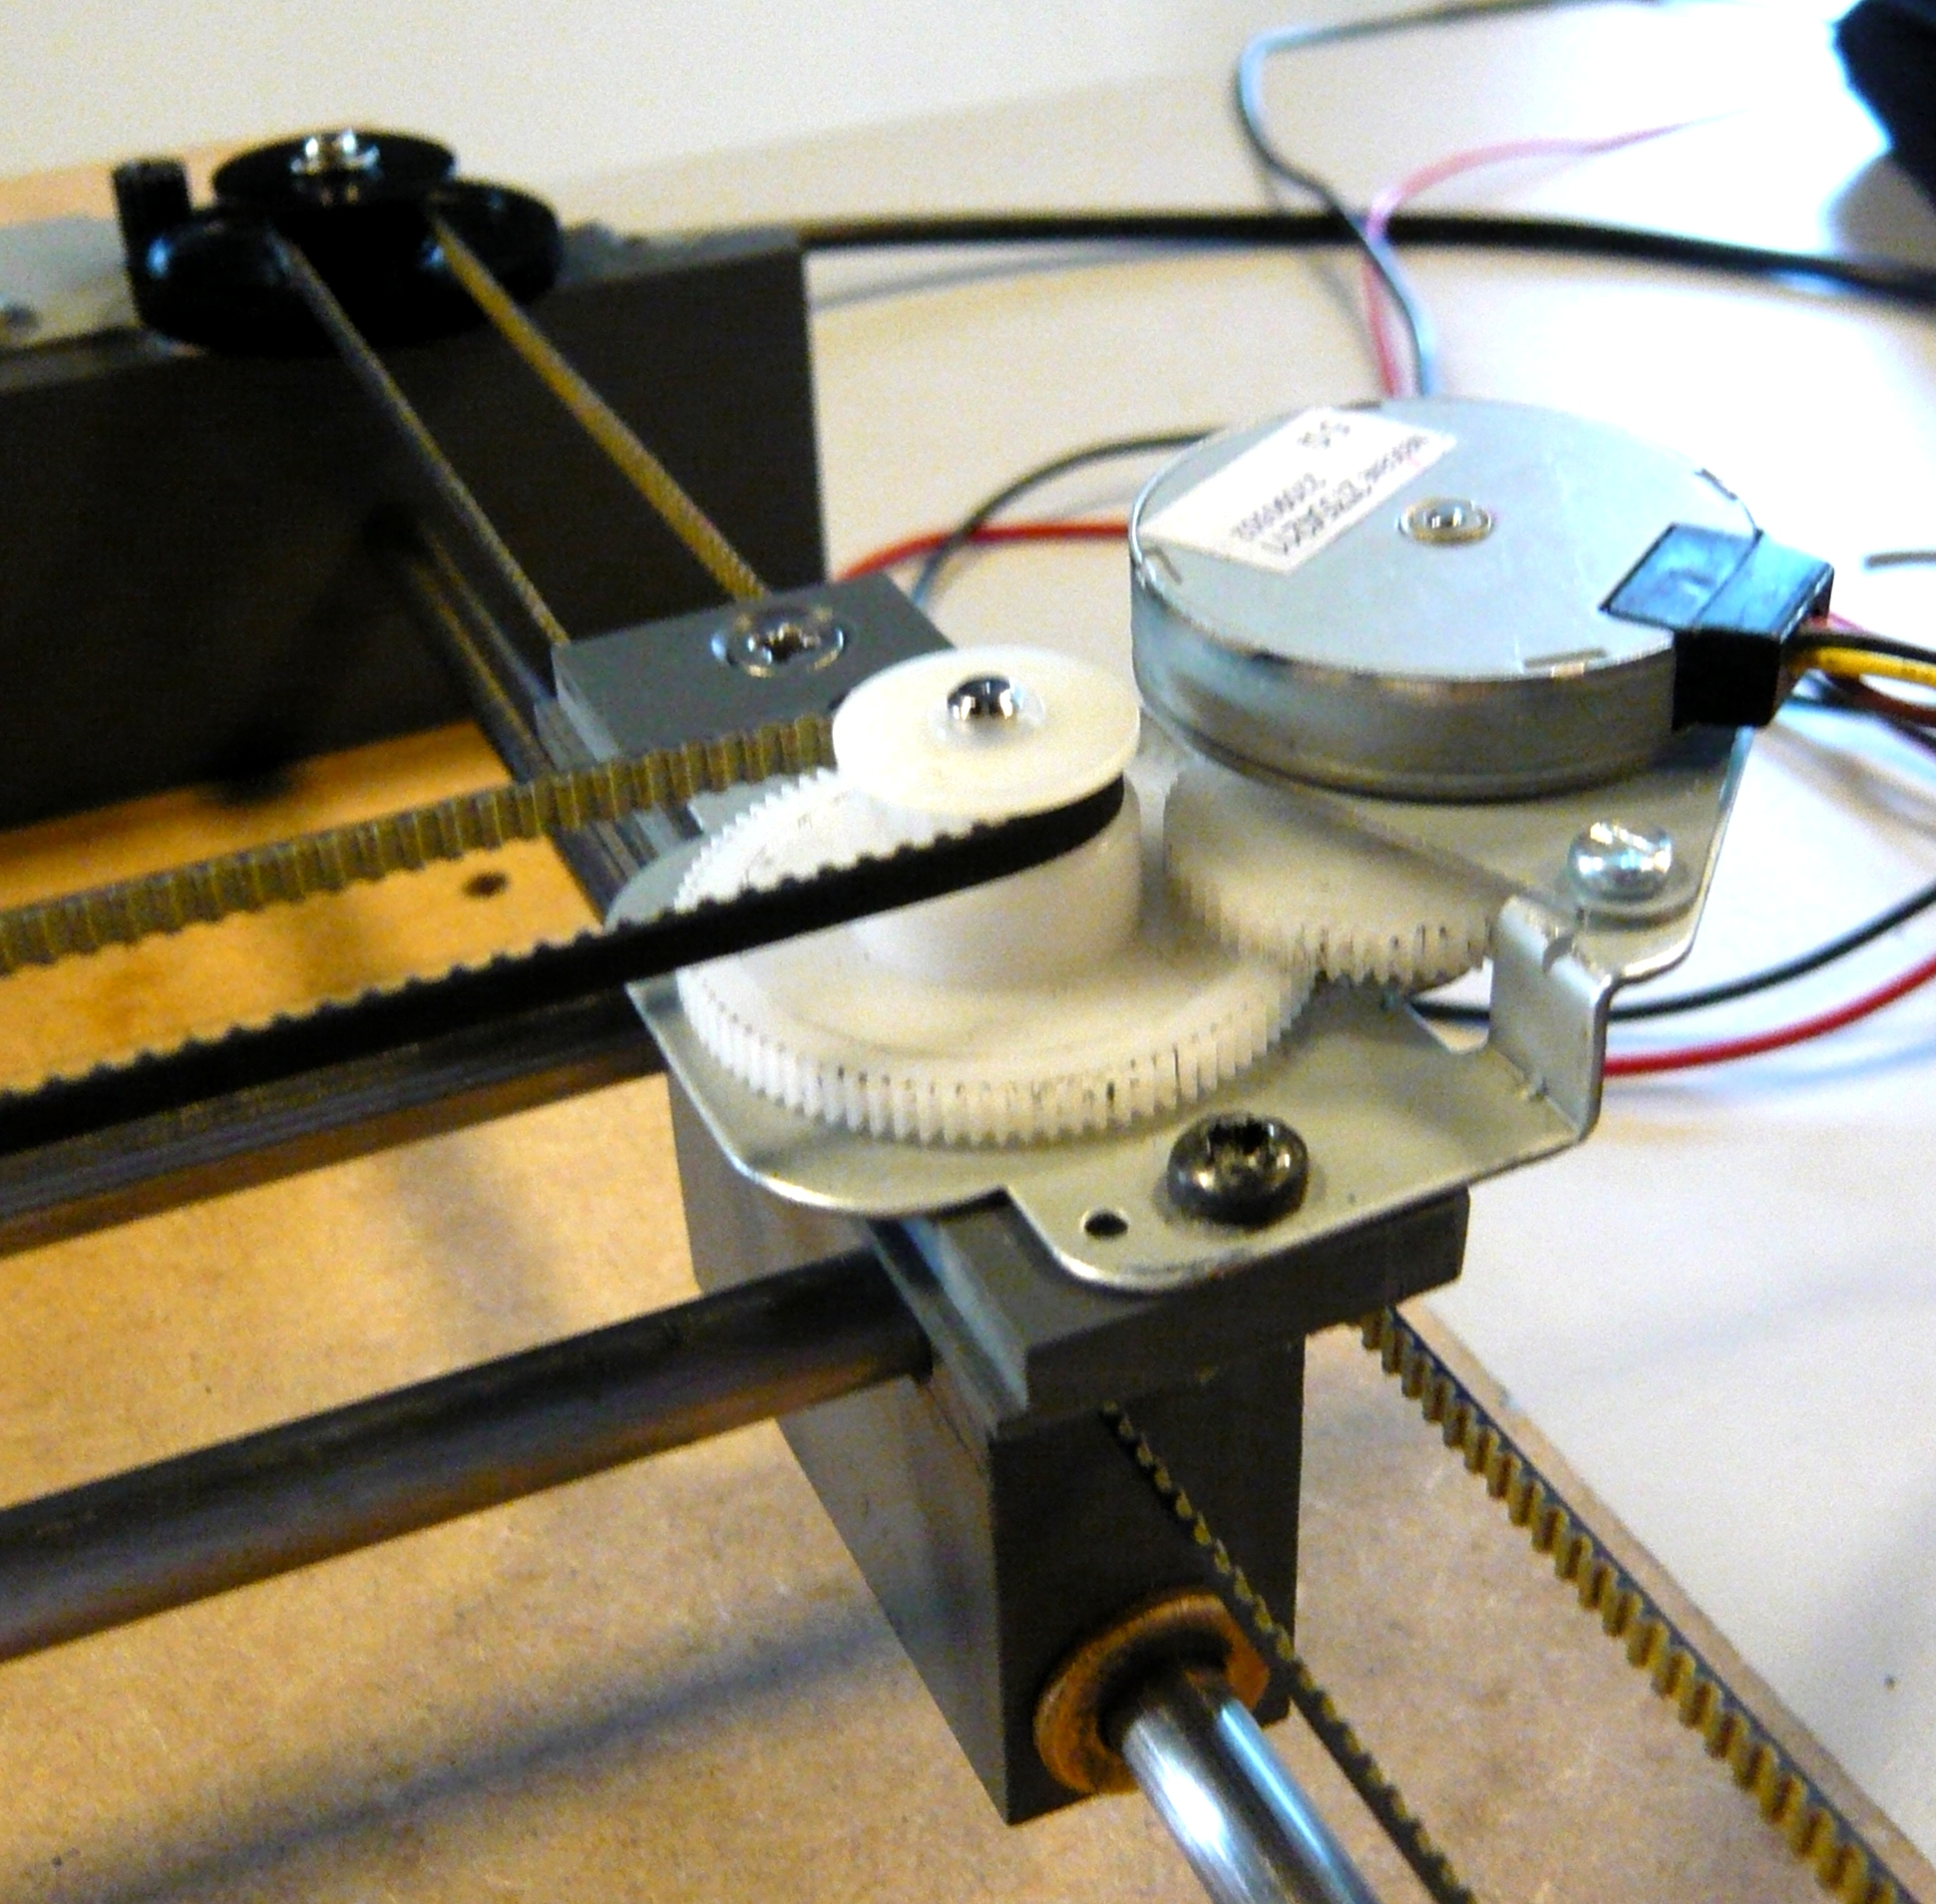
\includegraphics[width=\marginparwidth]{./img/y-motor}
  \captionof{figure}{Billede af y-motoren}
  \label{fig:y-motorimg}
}

\mnote{
  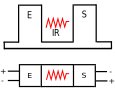
\includegraphics[width=\marginparwidth]{./img/fotogaffel}
  \captionof{figure}{Skitse af fotogaffel}
  \label{fig:fotogaffel-skitse}
}



%%% Local Variables: 
%%% mode: latex
%%% TeX-master: "../master"
%%% End: 
